\documentclass{article}

\usepackage[utf8]{inputenc} \usepackage[T1]{fontenc}

%%%%% 
\usepackage{graphicx} \usepackage{caption} \usepackage{subcaption}

% lock figure into place (H option of \begin{figure})
\usepackage{float}
  
% wrapping text around figures
\usepackage{wrapfig}

\usepackage[english]{babel}
\usepackage{setspace}

\usepackage{amsmath}
\usepackage{amssymb}
\usepackage{amsfonts}
\usepackage{amsopn}
\usepackage{braket}
\usepackage{bbm}
\usepackage{dsfont}
\usepackage{kpfonts}
% \usepackage{mathabx}

\parindent=0cm


% Various new commands that ease typesetting math even further
% \newcommand{\assign}{\ensuremath{\coloneq}}
% \newcommand{\rassign}{\ensuremath{\eqcolon}}
\newcommand{\assign}{\ensuremath{:=}}
\newcommand{\rassign}{\ensuremath{=:}}

\newcommand{\of}[1]{\ensuremath{\left( #1 \right)}}
\newcommand{\ofs}[1]{\ensuremath{\left( #1 \right)}}

\newcommand{\norm}[1]{\ensuremath{\| #1 \|}}

\newcommand{\tmop}[1]{\ensuremath{\operatorname{#1}}}

\newcommand{\id}{\ensuremath{\mathds{1}}}
% \newcommand{\id}{\ensuremath{I}}


\newcommand{\conj}[1]{\ensuremath{\overline{#1}}}

\newcommand{\T}{\ensuremath{{}^{\textnormal{T}}}}
\newcommand{\herm}{\ensuremath{{}^{\textnormal{H}}}}

\newcommand{\ft}[1]{\ensuremath{\mathcal{F}\left(#1\right)}}
\newcommand{\ift}[1]{\ensuremath{\mathcal{F}^{-1}\left(#1\right)}}

\newcommand{\fft}[1]{\ensuremath{\mathtt{FFT}\left(#1\right)}}
\newcommand{\ifft}[1]{\ensuremath{\mathtt{IFFT}\left(#1\right)}}

\newcommand{\dotp}[2]{\ensuremath{\langle #1 , #2 \rangle}}

\newcommand{\bigO}[1]{\ensuremath{\mathcal{O}\left( #1 \right)}}

\newcommand{\mat}[1]{\ensuremath{\mathbf{#1}}}

% multi-indices
\newcommand{\mindex}[1]{\ensuremath{\underline{#1}}}

\newcommand{\laplace}{\ensuremath{\operatorname{\Delta}}}

% EOF
  
\usepackage[ruled]{algorithm2e}

% Configure Algorithm2e
\DontPrintSemicolon
\SetKwInOut{Input}{Input}
\SetKwInOut{Output}{Output}

\def\code#1{\texttt{#1}}
\def\classname#1{\textit{#1}}
\def\filename#1{\textit{#1}}

\newtheorem*{definition}{Definition}

\begin{document}

\tableofcontents
\clearpage

\section{Basis Shape}

A \(D\)-dimensional
shape \(\mathfrak{K}\)
is a set of \emph{unordered} D-dimensional integer-tuples, also
referred to as \emph{nodes}.  A shape is suitable for our needs if it
satisfies:

\begin{equation}
  \label{eq:basis_shape_fundamental_property}
  \mindex{k} \in \mathfrak{K} \Rightarrow \forall
  \mindex{k}-\mindex{e}^d \in \mathfrak{K} \;\forall d \in \{d \;|\;k_d \geq 1\}
\end{equation}
That means, if an arbitrary node is part of the shape, then all nodes
in the backward cone are part of the shape too.

\subsection{Implementation}

\subsection{Shape Extension}

\begin{definition}
  Given a basis shape \( \mathfrak{K} \),
  the shape extension \( \overline{\mathfrak{K}} \) is defined by
  \begin{equation}
    \overline{\mathfrak{K}} := \mathfrak{K} \cup 
    \left\{\underline{k}' \colon \underline{k}' = \underline{k} + \underline{e}^d 
      \forall d \in \{1,\ldots,D\} \forall \underline{k} \in \mathfrak{K}\right\}
  \end{equation}
  where \( \underline{e}^d \) is the unit vector in direction \( d \).
\end{definition}

\begin{figure}[H]
  \begin{center}
    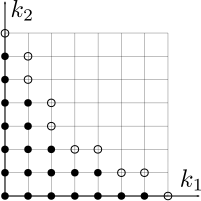
\includegraphics[width=0.5\linewidth]{shape_extension}
  \end{center}
  \caption{basic shape (filled bullets) and its extension (empty
    bullets)}
\end{figure}
\subsection{Shape Union}

\begin{definition}
  Given the shapes \( \mathfrak{K}_1, \ldots \mathfrak{K}_N \),
  the union of these shapes is defined by
  \begin{equation}
    union(\mathfrak{K}_1,\ldots,\mathfrak{K}_N) := \left\{ 
      \underline{k} \mid \exists i \in \{1, \ldots, N \} \colon \underline{k} \in \mathfrak{K}_i\right\}
  \end{equation}
\end{definition}

\section{Basis Shape Enumeration}



\begin{definition}
  A \( D \)-dimensional
  shape enumeration \( \mathfrak{K} \)
  is a set of ordered D-dimensional integer-tuples, also referred to
  as \emph{nodes}. It is a (bijective) mapping that orders all nodes
  of \( \mathfrak{K} \)
  and assigns the \(i\)-th node the ordinal \( (i-1) \).
\end{definition}

\subsection{Data Format}
Many algorithms, notable the evaluation of a \emph{Hagedorn wavepacket},
use recursive formulas in the form
\( c_{\mindex{k}} = f(c_{\mindex{k}-\mindex{e}^1}, \ldots,
c_{\mindex{k}-\mindex{e}^D}) \)
where \( c_{\mindex{k}} \)
is a value associated with the node \( \mindex{k} \)
and where \( \mindex{e}^d \)
is the unit vector in direction \( d \).
To simplify such algorithms, the class \classname{ShapeEnum} organizes a shape
into \emph{slices}.  The \( s \)-th
slice of a shape \( \mathfrak{K} \)
contains all nodes \( \mindex{k} \in \mathfrak{K} \)
that satisfy \( \sum_{d=1}^{D} k_d = s \) (Manhattan distance to origin).

\begin{figure}[H]
  \centering
  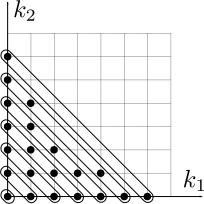
\includegraphics[]{shape_slicing}
  \caption{basic shape (filled bullets) and the slicing (rounded
    rectangles)}
\end{figure}

The implementation maintains for each slice an array containing all
nodes that are part of the slice. The user can decide at compile-time
which multi-index type to use: \\ \\ A suitable type must \dots
\begin{itemize}
\item \dots provide the same semantics as \code{std::array<int,D>}.
\item \dots specialize \code{std::less} to perform lexical comparison
  beginning on first index.
\item \dots specialize \code{std::equal\_to} and \code{std::hash}.
\end{itemize}
All nodes inside a slice are ordered according to \code{std::less} of
used multi-index type. Be aware that the implemented shape enumerator
currently assumes that \code{std::less} performes lexical
comparison. Other than that there is nothing inherent that obligates
lexical comparison.

\subsection{Enumerator}
A shape enumerator takes a shape object that describes which nodes it
contains. The enumerator converts that shape into a shape enumeration.

\subsection{Shape description}
There exists many ways to describe a shape. My basis shape enumerator
is able to enumerate a shape that defines its surface function and
minimum bounding box.

\begin{definition}[Surface functions of basis shapes]
  The \(D\) surface functions of an arbitrary \(D\)-dimensional shape are defined as:
  \begin{equation}
  s_{\alpha}(\mindex{n})=\max_{k_{\alpha}}
    \left\{\mindex{k} \in \mathfrak{K} \;|\;
      k_d = n_d \; \forall d \neq \alpha
    \right\}
    \label{eq:basis_shape_surface_function}
  \end{equation}
\end{definition}

These functions are well-defined because of the fundamental shape property
(\ref{eq:basis_shape_fundamental_property}).

The (explicit) functions \(s_{\alpha}\) are projections of an
implicit surface function \(S(\mindex{k}) = 0\) along the axis \(\alpha\).

\begin{definition}[Minimum bounding box of basis shapes]
  The minimum bounding box describes the smallest
  volume within which all lattice nodes lie.
  \begin{equation}
    L_{\alpha}=\max_{k_{\alpha}}\left\{\mindex{k} \in \mathfrak{K}\right\}
    \label{eq:basis_shape_bbox}
  \end{equation}
\end{definition}

\begin{figure}[H]
  \centering
  \begin{subfigure}[]{0.4\textwidth}
    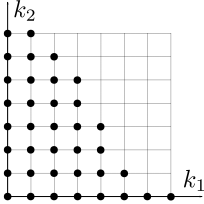
\includegraphics[width=1.0\textwidth]{shape_example}
    \label{fig:shape_example}
  \end{subfigure}
  ~
  \begin{subfigure}[]{0.5\textwidth}
    \begin{tabular}{|| c | c || c | c ||}
      \multicolumn{2}{|| c ||}{\( k_1 \) (first axis) } &
                                                          \multicolumn{2}{c ||}{\( k_2 \) (second axis) } \\
      \(\mindex{n}\) & \(s_1(\mindex{n})\) & \(\mindex{n}\) & \(s_2(\mindex{n})\) \\
      (?, 0) & 7 & (0, ?) & 7 \\
      (?, 1) & 5 & (1, ?) & 7 \\
      (?, 2) & 4 & (2, ?) & 6 \\
      (?, 3) & 4 & (3, ?) & 5 \\
      (?, 4) & 3 & (4, ?) & 3 \\
      (?, 5) & 3 & (5, ?) & 1 \\
      (?, 6) & 2 & (6, ?) & 0 \\
      (?, 7) & 1 & (7, ?) & 0 \\
      (?, 8) & \(-\infty\) & (8, ?) & \(-\infty\) \\
    \end{tabular}
  \end{subfigure}
  \caption{Example of a surface description of an arbitrary shape.}
\end{figure}

\subsection{Common Basis Shapes}
\begin{definition}[Hypercubic basis shape]
  Given the limits \(\mindex{K} \in \mathbb{N}^D\), a hypercubic shape is defined by

  \begin{equation}
    \label{eq:hypercubic_shape}
    \mathfrak{K}(D,\mindex{K}):=\left\{(k_1,\dots,k_D) \in \mathbb{N}_0^D \;|\; k_d < K_d \forall d\right\}
  \end{equation}
\end{definition}

We derive the surface functions by inserting (\ref{eq:hypercubic_shape}) into
equation
(\ref{eq:basis_shape_surface_function}).
\[
  s_{\alpha}(\mindex{n})=\max_{k_{\alpha}}\left\{(k_{\alpha}<K_{\alpha}) \;\land\;
    (n_d < K_d \;\forall d \neq \alpha)\right\}
\]

\begin{equation}
  s_{\alpha}(\mindex{n})=
  \begin{cases}
    k_{\alpha}-1 & n_d < K_d \;\forall d \neq \alpha \\
    -\infty & otherwise \\
  \end{cases}
\end{equation}

We retrieve the minimum bounding box by inserting (\ref{eq:hypercubic_shape}) into
equation
(\ref{eq:basis_shape_bbox}).

\[
L_{\alpha}=\max_{k_{\alpha}}\left\{k_{\alpha}<K_{\alpha}\right\}
\]

\begin{equation}
L_{\alpha}=K_{\alpha}-1
\end{equation}

\begin{definition}[Hyperbolic cut basis shape]
  Given the sparsity parameter \(S\), a hyperbolic cut shape is defined by
  \begin{equation}
    \mathfrak{K}(D,S):=\left\{(k_1,\dots,k_D) \in \mathbb{N}_0^D \;|\;\prod_{d=1}^D(k_d+1) \leq S\right\}
    \label{eq:hyperbolic_cut_shape}
  \end{equation}
\end{definition}

We derive the surface functions by inserting (\ref{eq:hyperbolic_cut_shape}) into
equation (\ref{eq:basis_shape_surface_function}).

\[
  s_{\alpha}(\mindex{n})=
  \max_{k_{\alpha}}\left\{(k_{\alpha}+1)\prod_{d \neq \alpha} (n_d+1) \leq S \right\} =
  \max_{k_{\alpha}}\left\{k_{\alpha}+1 \leq \frac{S}{\prod_{d \neq \alpha}(n_d+1)}\right\}
\]

\begin{equation}
s_{\alpha}(\mindex{n})=\frac{1}{\prod_{d \neq \alpha} (n_d+1)}-1
\end{equation}

We retrieve the minimum bounding box by inserting (\ref{eq:hyperbolic_cut_shape}) into
equation (\ref{eq:basis_shape_bbox}).

\[
  L_{\alpha}=\max_{k_{\alpha}}\left\{\prod_d(k_d+1) \leq S\right\} =
  \max_{k_{\alpha}}\left\{k_{\alpha}+1 \leq \frac{S}{\prod_{d \neq \alpha}(k_d+1)}\right\}
\]

\begin{equation}
L_{\alpha}=S-1
\end{equation}

\begin{definition}[Shape intersection]
  The intersection of the shapes \(\mathfrak{K}_{A}\) and \(\mathfrak{K}_{B}\) is defined by
  \begin{equation}
    \label{eq:basis_shape_intersection}
    \mathfrak{K}_{A \cap B}=\left\{\mindex{k} \;|\; \mindex{k} \in \mathfrak{K}_A \land
      \mindex{k} \in \mathfrak{K}_B
    \right\}
  \end{equation}
\end{definition}

Using equation (\ref{eq:basis_shape_surface_function}) and (\ref{eq:basis_shape_bbox})
one obtains the surface functions

\begin{equation}
  s_{\alpha}^{A \cap B}(\mindex{n}) = \min\{s_{\alpha}^A(\mindex{n}), s_{\alpha}^B(\mindex{n})\}
\end{equation}

and the minimum bounding box

\begin{equation}
  L_{\alpha}^{A \cap B} = \min\{L_{\alpha}^{A}, L_{\alpha}^{B}\}
\end{equation}

Remark: The \emph{limited hyperbolic cut shape} is an intersection of an
\emph{hypercubic shape} and a \emph{hyperbolic cut shape}.

\begin{definition}[Shape union]
  The union of the shapes \(\mathfrak{K}_{A}\) and \(\mathfrak{K}_{B}\) is defined by
  \begin{equation}
    \label{eq:basis_shape_intersection}
    \mathfrak{K}_{A \cup B}=\left\{\mindex{k} \;|\; \mindex{k} \in \mathfrak{K}_A \lor
      \mindex{k} \in \mathfrak{K}_B
    \right\}
  \end{equation}
\end{definition}

Using equation (\ref{eq:basis_shape_surface_function}) and (\ref{eq:basis_shape_bbox})
one obtains the surface functions

\begin{equation}
  s_{\alpha}^{A \cup B}(\mindex{n}) = \max\{s_{\alpha}^A(\mindex{n}), s_{\alpha}^B(\mindex{n})\}
\end{equation}

and the minimum bounding box

\begin{equation}
  L_{\alpha}^{A \cup B} = \max\{L_{\alpha}^{A}, L_{\alpha}^{B}\}
\end{equation}

\subsection{Basis shape enumeration}
A basis shape just tells you whether it contains a specific node. But
for many algorithms, one needs to associate values \(c_{\mindex{k}}\) with shape
nodes \(\mindex{k}\). One way to do that is using a dictionary. But it is simpler to
enumerate all nodes in a shape.  This way one is able to keep those
values in an array, ordered according to the enumeration.

Knowing the \emph{surface} and \emph{bounding volume} of a shape, the
enumerator lexically enumerates all nodes inside the shape. All nodes
are subsequently put into the proper shape.

\begin{figure}[H]
  \centering
  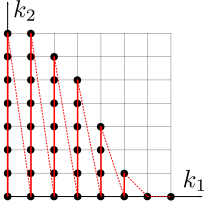
\includegraphics[]{shape_enumerator}
  \caption{enumerator passage through a description of a 2D-shape}
  \label{fig:shape_example}
\end{figure}

\begin{algorithm}[H]
  \For{\(x \leftarrow 0\) \KwTo shape.surface(\(\{0,0,0\}\),\(0\))}{
    \For{\(y \leftarrow 0\) \KwTo shape.surface(\(\{x,0,0\}\),\(1\))}{
      \For{\(z \leftarrow 0\) \KwTo shape.surface(\(\{x,y,0\}\),\(2\))}{
        slice[x+y+z].pushback(\(\{x,y,z\}\)); } } }
  \caption{Enumerator passage through a 3-dimensional shape.}
\end{algorithm}

\subsection{Implementation}

The file \emph{waveblocks/shape\_enum.hpp} provides the implementation of the shape enumeration.

\begin{verbatim}
template<dim_t D, class MultiIndex, class S>
class DefaultShapeEnumeration;
\end{verbatim}

\begin{description}
\item[D] number of dimensions
\item[MultiIndex] type to internally represent multi-indices
\item[S] shape description
\end{description}

\subsubsection{Internal multi-index representation}
The default shape enumeration stores all nodes in a vector. Since
using \emph{std::array\textless int,D\textgreater} would use a lot of
memory, the default enumeration exposes a template parameter to define
a better type. \\ \\ A suitable type must \dots
\begin{itemize}
\item provide the same semantics as \emph{std::array\textless
    int,D\textgreater}
\item specialize \emph{std::less} to perform lexical comparison
\item specialize \emph{std::equal\_to}
\item specialize \emph{std::hash}
\end{itemize}

\subsubsection{Shape definition}
A shape definition class provides two member functions:

\begin{itemize}
\item
\begin{verbatim}
int limit(dim_t axis) const;
\end{verbatim}
  This member function returns for a given axis \( j \)
  an as small as possible limit \( L_j \) such that:
  \[ \forall \boldsymbol{k} \in \mathfrak{K} \,\colon\; k_j \leq
    L_j \]

\item
\begin{verbatim}
template<class MultiIndex>
int limit(const MultiIndex &base_node, dim_t axis) const;
\end{verbatim}
  This member function for a given axis \( j \)
  and a given base node \( \boldsymbol{n} \)
  (whose \( j \)-th
  entry is zero) the largest element \( k^\star \) that satisfies:
  \[ \boldsymbol{k} \in \mathfrak{K}, \; k_i =
    \begin{cases}
      n_i,& i \neq j\\
      k^\star, & i = j
    \end{cases}
  \]

\end{itemize}

\subsubsection{Queries}
The default shape enumeration stores all multi-indices in a vector
using lexical ordering. The query \emph{ordinal} \(\rightarrow\)
\emph{multi-index} is therefore trivial. The query \emph{multi-index}
\(\rightarrow\)
\emph{ordinal} is done using binary search. Alternatively this
implementation can be forced to use \emph{std::unordered\_map} but
performance tests revealed that a dictionary is slightly slower than
binary seach.

\section{Hagedorn Wavepacket}
\subsection{Scalar Wavepackets}
A scalar Hagedorn wavepacket
\[
  \Phi_{\mathfrak{K}}^{\varepsilon}[\Pi] = e^{iS\pi} \sum_{\underline{k} \in
    \mathfrak{K}}^{} c_{\underline{k}} \phi_{\underline{k}} \]
is represented by a tuple
\[ \Phi := \left( \varepsilon, \Pi, \mathfrak{K}, \boldsymbol{c}
  \right) \]
where \(\varepsilon\) is the semi-classical scaling parameter.
\(\Pi\) is the Hagedorn parameter set
\[ \Pi := \left( \vec{p}, \vec{q}, \mat{P}, \mat{Q}, S \right) \]

\subsection{Vectorial Wavepackets}
Vectorial Hagedorn wavepackets \(\Psi\) have multiple components \(\Phi_i\):
\[
  \Psi(\vec{x}) :=
  \begin{pmatrix}
    \Phi_1(\vec{x}) \\
    \Phi_2(\vec{x}) \\
    \vdots \\
    \Phi_N(\vec{x}) \\
  \end{pmatrix}
\]
The components \(\Phi_i\) itself are plain scalar wavepackets.
They have the same scaling parameter \(\varepsilon\) in common but
the Hagedorn parameter set and the basis shape may differ depending on
the concrete type. \\
Common vectorial wavepacket types are:
\begin{description}
\item[Inhomogeneous wavepacket]
  The inhomogeneous wavepacket is the most general case as its components only share
  the scaling parameter \(\varepsilon\).
  \[
    \Phi_i := (\varepsilon, \Pi_i, \mathfrak{K}_i, c_i) \] \[
    \Psi := \left(\varepsilon, 
    \begin{pmatrix}
      (\Pi_1, \mathfrak{K}_1, c_1) \\
      \vdots \\
      (\Pi_N, \mathfrak{K}_N, c_N) \\
    \end{pmatrix}\right)
  \]
\item[Homogeneous wavepackets]
  A homogeneous wavepacket is a special case of the inhomogeneous wavepacket
  since all components share the same Hagedorn parameter set \(\Pi\).
  \[
    \Phi_i := (\varepsilon, \Pi, \mathfrak{K}_i, c_i) \] \[
    \Psi := \left(\varepsilon, \Pi,
    \begin{pmatrix}
      (\mathfrak{K}_1, c_1) \\
      \vdots \\
      (\mathfrak{K}_N, c_N) \\
    \end{pmatrix}\right)
  \]
\item[Gradient]
  The gradient of a scalar Hagedorn wavepacket can be represented using a vectorial Hagedorn
  wavepacket. All components share the same Hagedorn parameter set and the
  same basis shape (which is an extension of the original wavepacket's basis shape).
  \[
    \frac{\partial \Phi}{\partial x_i} := (\varepsilon, \Pi, \mathfrak{K}_{ext}, c'_i) \] \[
    \vec{\nabla} \Phi := \left(\varepsilon, \Pi, \mathfrak{K}_{ext},
    \begin{pmatrix}
      (c'_1) \\
      \vdots \\
      (c'_D) \\
    \end{pmatrix}\right)
  \]
\end{description}


\subsection{Class Diagram}

\begin{figure}[H]
  \centering
  \includegraphics[width=1.0\textwidth]{hawp_inheritance}
  \caption{Wavepacket classes and the inheritance hierarchy}
  \label{fig:hawp_inheritance}
\end{figure}

\subsubsection{Scalar wavepacket classes}

The superclass of all (scalar) Hagedorn wavepackets is \emph{AbstractScalarHaWp}.
It provides read-only access to its parameters through its (abstract) virtual
member functions \emph{eps()}, \emph{parameters()}, \emph{shape()} and \emph{coefficients()}.

It provides following functions as a service:
\begin{description}
\item[evaluate(grid)]
This function gathers the wavepacket parameters \(\varepsilon\), \(\Pi\), \(\mathfrak{K}\) and \(c\) 
through the mentioned virtual member functions \emph{eps()}, \emph{parameters()},
\emph{shape()} and \emph{coefficients()}. Using these parameters it evaluates the wavepacket \(\Phi(\vec{x})\)
on the grid nodes \(\vec{x}\).
\item[evaluate\_basis(grid)]
  It evaluates all basis functions \(\phi_{\mindex{k}}(\vec{x})\) on the grid \(\vec{x}\)
for all \(\mindex{k} \in \mathfrak{K}\). This function is not dependent on the coefficients
\(c_{\mindex{k}}\), therefore I created a further abstract class \emph{AbstractScalarHaWpBasis} that
only contains the parameters \(\varepsilon\), \(\Pi\) and \(\mathfrak{K}\). \emph{AbstractScalarHaWp}
inherits from this base class and extends it with the coefficients \(c_{\mindex{k}}\).
\item[extended\_shape()]
  This non-virtual function returns the basis shape extension \(\mathfrak{K}_{ext}\)
  of the current basis shape \(\mathfrak{K}\). It is used for the gradient computation.
  Creating a basis shape extension is expensive, therefore \(\mathfrak{K}_{ext}\) is cached.
\end{description}

\subsubsection{Vectorial wavepacket classes}
Vectorial wavepacket class are implemented as a composition of scalar wavepackets.
Common aspects are stored in the composition class while different aspects are
stored in the component class.
\par
\emph{Example: } All components of a homogeneous wavepacket share the Hagedorn parameter
set \(\Pi\). Therefore \(\Pi\) is stored inside the composition class \emph{HomogeneousHaWp}.
The component classes \emph{HomogeneousHaWp::Component} only refer to \(\Pi\) to fulfill the contract
of the abstract superclass \emph{AbstractScalarHaWp}.

\subsubsection{Rationale}

\textbf{Abstract superclasses don't provide writeable access to parameters.} \par
Editing parameters of a superclass can have unwanted side-effects
you have no control over since subclasses may share parameters across many wavepackets.
A nice example is an inhomogeneous wavepacket: All components refer to the same Hagedorn parameter set
and scaling parameter \(\varepsilon\).
However concrete subclasses like \emph{ScalarHaWp}, \emph{HomogeneousHaWp}, etc. provide writeable
access to its parameters. This is safe because you know at \emph{compile-time} that you are working with
an homogeneous wavepacket thus you know that if you change the parameter set of one compile, you change
all components. This side-effects are controllable.

\bigskip

\textbf{Scalar and Vectorial wavepackets don't have a common superclass.} \par
The python version actually does that. It proved to be a bad choice.
The problem is that evaluation and parameter access functions would yield
results with different shapes dependent on the actual wavepacket type.
As an example, the function \emph{evaluate()} of a scalar wavepacket yields a scalar value, while
applied on a vectorial wavepacket, this function will yield a vector.
In python this behaviour is halfway manageable because of python's high flexible type system
and numpy's broadcasting operations.
However, dealing with such a behaviour is very hard in C++.
Therefore scalar and vectorial wavepacket don't have a common superclass.

\bigskip

\textbf{There is no dedicated class to represent a gradient of a vectorial wavepacket.} \par
Applying the gradient operator to a vectorial wavepacket is trivial. Just apply it
to its components:
\[\nabla \Psi \equiv
\begin{pmatrix}
  \nabla \Phi_1 \\
  \vdots \\
  \nabla \Phi_N \\
\end{pmatrix}
\]
It is an overkill to introduce a new class, just to replace a for-loop.
Furthermore, storing all coefficients of \(\vec{\nabla}\Psi\) occupies \(\mathcal{O}(D \cdot N \cdot M)\) space.
Using a basis shape of a realistic size \(M=1'000'000\), and wavepacket
dimensionality \(D=10\), one can easily run out of memory.

\subsection{Basis Evaluation}

All basis values are evaluated recursively. Once we have the basis
value at an anchor node \(\mindex{k}\) and the basis values of all
backward neighbours \(\mindex{k}-\mindex{e}^d\), we can compute all
forward neighbours by

\begin{equation}
  \begin{pmatrix}
    \phi_{\mindex{k}+\mindex{e}^1} \\
    \vdots \\
    \phi_{\mindex{k}+\mindex{e}^D}
  \end{pmatrix}
  = \left(
    \sqrt{\frac{2}{\varepsilon^2}} \mat{Q}^\mathrm{-1} (\vec{x}-\vec{q}) \phi_{\mindex{k}}
    - \mat{Q}^\mathrm{H} \mat{Q}^\mathrm{-T}
    \begin{pmatrix}
      \sqrt{k_1} \phi_{\mindex{k}-\mindex{e}^1} \\
      \vdots \\
      \sqrt{k_D} \phi_{\mindex{k}-\mindex{e}^D}
    \end{pmatrix}
  \right)
  \oslash
  \begin{pmatrix}
    \sqrt{k_1+1}\\
    \vdots \\
    \sqrt{k_D+1}
  \end{pmatrix}
\end{equation}

where the operator \(\oslash\) denotes component-wise division.

\begin{figure}[H]
  \centering
  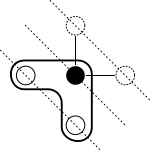
\includegraphics[]{basis_eval_stencil}
  \caption{Stencil of a 2-dimensional wavepacket}
\end{figure}

The root node \(\mindex{0}\) is evaluated by

\begin{equation}
  \label{eq:phi0_Dd}
  \phi_{\mindex{0}}[\Pi]\left(\vec{x}\right)
  \assign
  (\pi\varepsilon^2)^{-\frac{D}{4}} (\det\mat{Q})^{-\frac{1}{2}}
  \exp \left( \frac{i}{2\varepsilon^2}
    \dotp{(\vec{x}-\vec{q})}{\mat{P}\mat{Q}^\mathrm{-1}(\vec{x}-\vec{q})}
    + \frac{i}{\varepsilon^2} \dotp{\vec{p}}{(\vec{x}-\vec{q})}
  \right)
\end{equation}

Basis values of lattice nodes with some negative indices are zero.

\subsubsection{Implementation}
There are many possibilities to implement this recursion scheme. One
possibility is.
\begin{description}
\item[Scatter Type Strategy] We maintains a queue of already computed
  anchor nodes \(\mindex{k}\).  We subsequently remove one feasible(!)
  entry of this queue, compute the basis values of all forward
  neighbours \(\mindex{k}-\mindex{e}^d\) and put those nodes into the
  queue.  To eliminate multiple evaluation of some basis nodes, we
  need to check whether a forward neighbour already has been computed
  using a set.  Therefore the scatter type strategy is very bad suited
  for multi-threading since threads need to synchronize access to this
  set.
\item[Gather Type Strategy] We maintain a queue of not yet computed
  forward neighbours \(\mindex{k}-\mindex{e}^d\). Entries of this queue
  have at least one backward neighbour (called \emph{anchor node})
  that already has been computed.  We subsequently remove one entry of
  the queue (called \emph{child node}) and compute its basis value.
  Then we check, whether \emph{all} backward neighbours of the child
  node are computed. If this is the case put all forward neighbours of
  the child node into he queue.
\end{description}

A straight-forward implementation has at least one of following
difficulties that require complex data structures such as dictionaries
or would require excessive thread synchroniztation if we want
parallelisation:
\begin{description}
\item[A] We need to ensure that an already computed node is a valid
  anchor node (all backward neighbours has been computed too) so that
  we can compute its forward neighbours.
\item[B] We need to avoid multiple evaluation of the same node.
\end{description}

My rather simple solution is to split the shape into splices.  The
\(s\)-th slice contains all nodes \(\mindex{k}\) that fulfill
\( \sum_{d=1}^{D} k_d = s \).

\begin{figure}[H]
  \begin{center}
    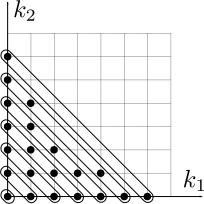
\includegraphics{shape_slicing}
  \end{center}
\end{figure}

Using an \emph{adequate} \footnote{See section \emph{Basic Shape}}
shape, the recusion scheme implies that if we had computed all basis
values of the parent slice \( \mathfrak{K}^{s-1} \) and of the current
slice \( \mathfrak{K}^{s} \), then we can compute all basis values of
the child slice \( \mathfrak{K}^{s+1} \) without having difficulty
\textbf{A}.  Furthermore if we use the gather type strategy where we
iterate through the child slice and compute its basis values, we
automatically avoid difficulty \textbf{B}.

My solution has two compelling advantages:
\begin{description}
\item[Simple data structures] We can keep our computed basis value in
  an array separated slice by slice. We need a \emph{shape
    enumeration} that maps shape nodes to ordinals used as array
  offsets.
\item[Easy parallelisation] I implemented the gather type strategy
  therefore one could simply split the iteration over the child slice
  using \code{pragma omp parallel for}. All previous slices has been
  completely computed therefore the only synchronisation mechanism
  needed is a barrier at the end of the child slice.
\end{description}

\begin{algorithm}[H]
  \Input{number of slices \(S\)}
  \Input{shape enumeration (slices)
    \(\mathfrak{K} = \left(\mathfrak{K}^0, \ldots,
      \mathfrak{K}^{S-1}\right)\)}
  \Output{basis values on each slice
    \(\phi = \left(\phi^0, \ldots, \phi^{S-1}\right)\)} initialization\;
  \(\phi^-, \phi, \phi^+ \gets \emptyset \)\;
 
  \emph{Compute ground state}\;
 
  \( \gets \left\{ \phi_{\mindex{0}}[\Pi](\vec{x}) \right\} \)\;
  \emph{Loop over all slices}\;
  \ForEach{\(\mathfrak{K}^s \in \mathfrak{K}\)}{ \emph{Loop over all
      nodes of next slice}\;
    \For{\(\mindex{k}^{s+1} \in \mathfrak{K}^{s+1}\)}{ \emph{find
        suitable anchor node (in current slice)}\;
      \(\alpha \gets undef \)\\
      \For{\(d \in \{1,\ldots,D\}\)}{ \If{\(k^{s+1}_{d} > 0\)}{
          \(\alpha \gets d\)\; } } \emph{here is our anchor node
        \(\mindex{k}^{s}\)}\;
      \(\mindex{k}^{s} \gets \mindex{k}^{s+1} - \mindex{e}^\alpha\)\;
    
      \emph{compute contribution of anchor node}\;
      \(a \gets
      \frac{\sqrt{2}}{\varepsilon}\left(\mat{Q}^\mathrm{-1}(\vec{x}-\vec{q})\right)_\alpha\phi^{s}_{\mindex{k}}\)
    
      \emph{compute contribution of anchor node's backward
        neighbours}\; \(b \gets 0\)\;
      \For{\(d \in \{1,\ldots,D\}\)}{
        \If{\(k^{s}_{d} > 0\)}{
          \(b \gets b + \sqrt{k^{s}_d}
          \left(\mat{Q}^{\mathrm{H}}\mat{Q}^{\mathrm{-T}}\right)_{\alpha
            d} \phi^{s-1}_{\mindex{k}^{s}-\mindex{e}^d}\)\; } }
    
      \emph{compute value of basis at \(\mindex{k}^{s+1}\)}\;
      \(\phi^{s+1}_{\mindex{k}^{s+1}} \gets
      \frac{a-b}{\sqrt{1+k^{s}_\alpha}} \) } }
  \caption{Recursive basis evaluation of hagedorn wavepacket}
\end{algorithm}



\subsection{Gradient Computation}
Applying the gradient operator to a scalar \(D\)-dimensional Hagedorn Wavepacket 
\( \Phi = \left( \varepsilon, \Pi, \mathfrak{K}, c \right)\)
yields a vectorial Hagedorn Wavepacket \(\Psi=\vec{\nabla}\Phi\) with \(D\) components.
The wavepacket gradient \(\Psi\) has the same parameterset \(\Pi\) as the original wavepacket \(\Phi\),
but has a new coefficients set \(c'\) given by

\begin{equation}
  \label{eq:compute_grad_coeff}
  c'_{\mindex{k}}=c_{\mindex{k}}\vec{p}+\sqrt{\frac{\varepsilon^2}{2}}
  \left(\mat{\overline{P}}
    \begin{pmatrix}
      c_{\mindex{k}+\mindex{e}^1}\sqrt{k_1+1} \\
      \vdots \\
      c_{\mindex{k}+\mindex{e}^D}\sqrt{k_D+1} \\
    \end{pmatrix}
    +\mat{P}
    \begin{pmatrix}
      c_{\mindex{k}-\mindex{e}^1}\sqrt{k_1} \\
      \vdots \\
      c_{\mindex{k}-\mindex{e}^D}\sqrt{k_D} \\
    \end{pmatrix}
  \right)
\end{equation}

Some wavepacket gradient coefficients outside of the original basis shape are non-zero.
Thus the wavepacket gradient needs a new parameter set \(\mathfrak{k}_{ext}\)
with the following property

\begin{equation}
  \label{eq:shape_extension_requirement}
  \mindex{k} \in \mathfrak{K} \Rightarrow
  \left(
     \mindex{k} \in \mathfrak{K}_{ext}
  \right)
  \wedge
  \left(
    \mindex{k}+\mindex{e}^1 \in \mathfrak{K}_{ext}
    \wedge \dots \wedge
    \mindex{k}+\mindex{e}^D \in \mathfrak{K}_{ext}
  \right)
\end{equation}

\subsubsection{How it was done in Python}
The original python code uses a \emph{scatter-type strategy}:
It loops over all \(\mindex{k} \in \mathfrak{K}\) and computes its contribution
to its neighbours in \(\mathfrak{K}_{ext}\). The reason to use this strategy is,
how the shape extension \(\mathfrak{K}_{ext}\) is implemented. It contains far more
entries than required by equation \eqref{eq:shape_extension_requirement}.
Since the scatter-type strategy loops over \(\mathfrak{K}\) and
not over the oversized \(\mathfrak{K}_{ext}\), no computation power is wasted.

\begin{figure}[H]
  \centering
  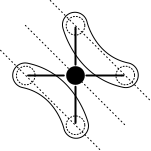
\includegraphics{grad_scatter_stencil}
  \caption{Stencil of scatter-type algorithm}
  \label{fig:grad_scatter_stencil}
\end{figure}

\subsubsection{How I have implemented it}
As my shape extension \(\mathfrak{K}_{ext}\) implementation only contains
nodes that are really required by equation \eqref{eq:shape_extension_requirement},
there is no necessity for me to use the scatter type strategy.
Instead my implementation uses the \emph{gather-type strategy}: It loops over all
\(\mindex{k} \in \mathfrak{K}_{ext}\), gathers the values of its contributors
and finally computes the new coefficients \(c'_{\mindex{k}}\) according to equation
\eqref{eq:compute_grad_coeff}.
I decided to use this strategy because it is much easier to parallelize.
For each node, the program just writes to one instead of \(2D\) locations.
This greatly simplifies parallelization.

\begin{figure}[H]
  \centering
  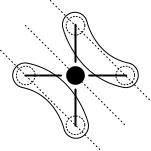
\includegraphics{grad_gather_stencil}
  \caption{Stencil of gather-type algorithm}
  \label{fig:grad_gather_stencil}
\end{figure}

\begin{algorithm}[H]
  \Input{\(\varepsilon\)}
  \Input{wavepacket dimension \(D\)}
  \Input{wavepacket parameters \(\Pi=(\vec{q},\vec{p},\mat{Q},\mat{P}))\)}
  \Input{shape enumeration \(\mathfrak{K}\)}
  \Input{shape extension enumeration \(\mathfrak{K}_{ext}\)}
  \Input{coefficients (scalars) of wavepacket \(\boldsymbol{c}\)}
  \Output{coefficients (\(D\)-dimensional vectors) of wavepacket gradient \(\boldsymbol{\vec{c_\nabla}}\)}
  \For{\(\mindex{k} \in \mathfrak{K}_{ext} \)}{
    \emph{compute contribution of center node}\;
    \(m \leftarrow 0\)\;
    \If{\(\mindex{k} \in \mathfrak{K}\)}{
      \(m \leftarrow c_{\mindex{k}}\)\;
    }

    \emph{compute contribution of backward neighbours}\;
    \(\vec{b} \leftarrow 0\)\;
    \For{\(d \in \{1,\ldots,D\}\)}{
      \If{\(\mindex{k}-\mindex{e}^d \in \mathfrak{K}\)}{
        \(b_d \leftarrow \sqrt{k_d}c_{\mindex{k}-\mindex{e}^d}\)\;
      }
    }

    \emph{compute contribution of forward neighbours}\;
    \(\vec{f} \leftarrow 0\)\;
    \For{\(d \in \{1,\ldots,D\}\)}{
      \If{\(\mindex{k}+\mindex{e}^d \in \mathfrak{K}\)}{
        \(f_d \leftarrow \sqrt{k_d+1}c_{\mindex{k}+\mindex{e}^d}\)\;
      }
    }

    \emph{merge contributions of every node to get the coefficients of the gradient}\;
    \(\vec{c_{\nabla,\mindex{k}}} \leftarrow m\vec{p}+\frac{\varepsilon}{\sqrt{2}}(\mat{\overline{P}}\vec{f}+\mat{P}\vec{b})\)
  }
  \caption{Computes coefficients of the wavepacket gradient \(\vec{\nabla} \Phi\)}
\end{algorithm}

\end{document}
